% Boilerplate and packages
\documentclass[a4paper,12pt]{article}
\usepackage{latexsym, amsmath, amssymb, amsfonts}
\usepackage{graphicx, float}
\graphicspath{{figures/}}
\usepackage[utf8]{inputenc}
\usepackage{polski}
\usepackage{XCharter}
\usepackage{geometry}
\geometry{
 a4paper,
 left=30mm,
 right=30mm,
 top=30mm,
 bottom=30mm
}

\title{Funkcje trygonometryczne}
\author{Zachariasz Jażdżewski}
\frenchspacing
\setlength{\parindent}{0pt}

% Actual document
\begin{document}
\maketitle

\tableofcontents

\section{Opis}

\textbf{Funkcje trygonometryczne} – zbiór kilku funkcji matematycznych wyrażających między innymi stosunki między długościami boków trójkąta prostokątnego zależnie od miar jego kątów wewnętrznych. Funkcje te wywodzą się z geometrii, jednak są rozpatrywane także w oderwaniu od niej, dla różnych argumentów rzeczywistych i innych zespolonych. Umożliwia to analiza matematyczna, w której opisano te funkcje szeregami potęgowymi, co prowadzi do uogólnień na inne dziedziny. Powstały też inne definicje, oparte np. na równaniach różniczkowych.\\

Do funkcji trygonometrycznych zalicza się przede wszystkim sinus, kosinus i tangens, a także kotangens, sekans, kosekans i kilka innych, wspominanych rzadziej. Funkcje trygonometryczne stosuje się w różnych działach matematyki, innych naukach ścisłych i technice. Funkcje te bada trygonometria, a konkretniej goniometria.

\newpage

\section{Wykresy funkcji}

Krzywe, będące wykresami funkcji sinus, cosinus, tangens, cotangens nazywa się odpowiednio: sinusoidą, cosinusoidą, tangensoidą i cotangensoidą. 

% Wykres funkcji sinus
\begin{figure}[h]
    \centering
    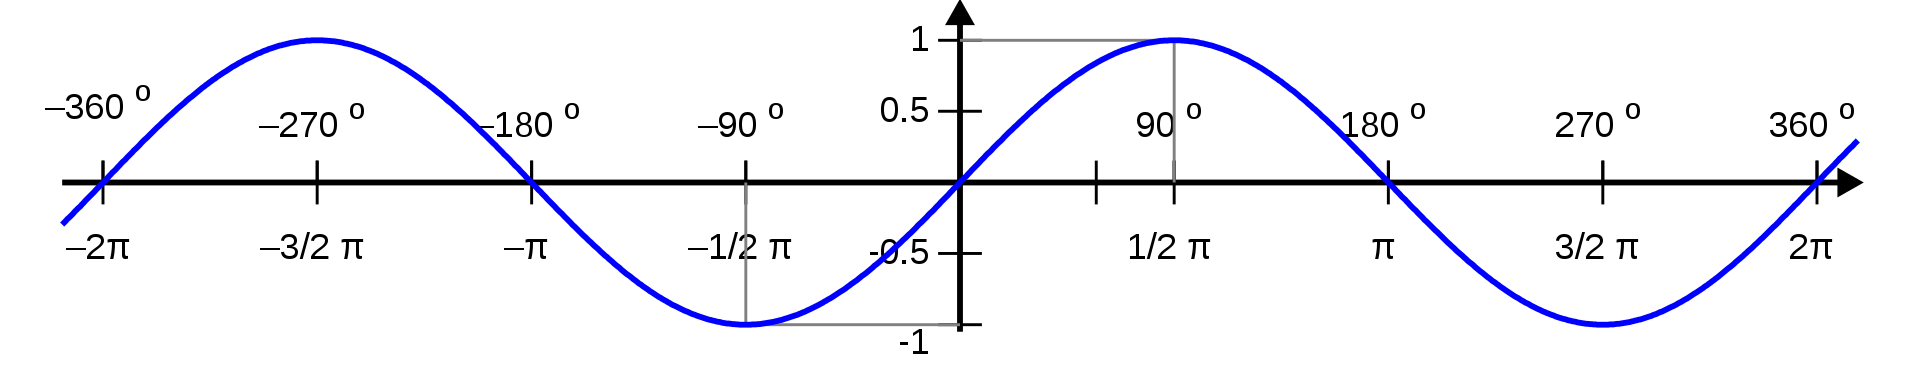
\includegraphics[width=\textwidth]{Sin_proportional.png}
    \caption{Sinusoida: wykres funkcji $y = \sin x$}
    \label{fig:wykres-sinus}
\end{figure}

% Wykres funkcji cosinus
\begin{figure}[h]
    \centering
    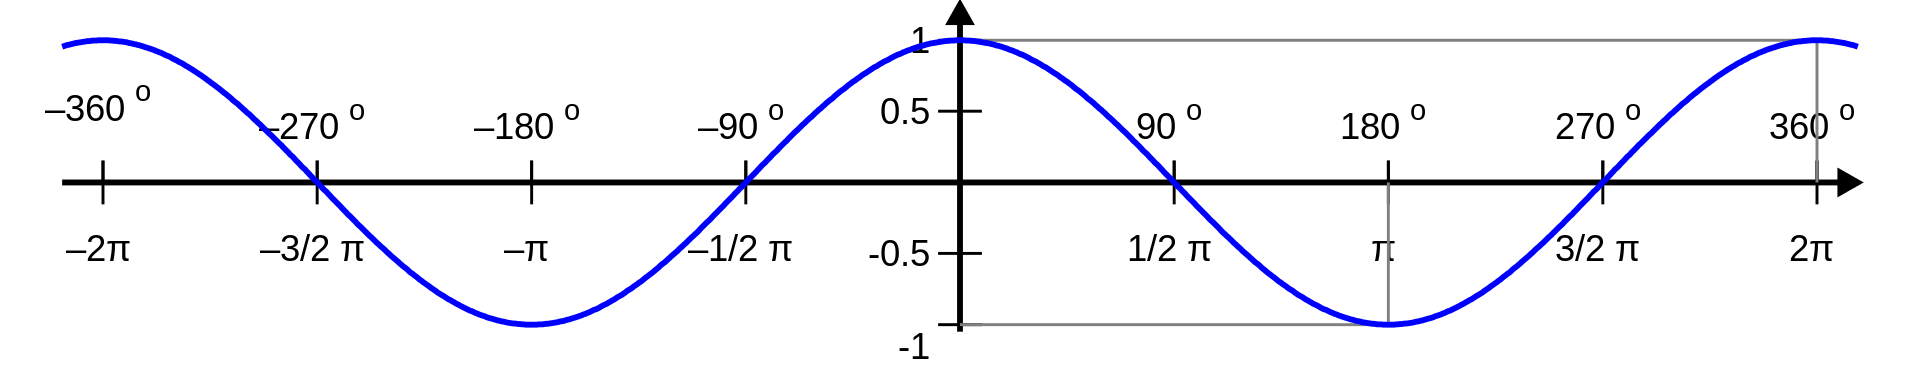
\includegraphics[width=\textwidth]{Cos_proportional.png}
    \caption{Sinusoida: wykres funkcji $y = \cos x$}
    \label{fig:wykres-cosinus}
\end{figure}


% Wykresy funkcji tangens i cotangens
\begin{figure}[h]
    \begin{minipage}{0.5\textwidth}
        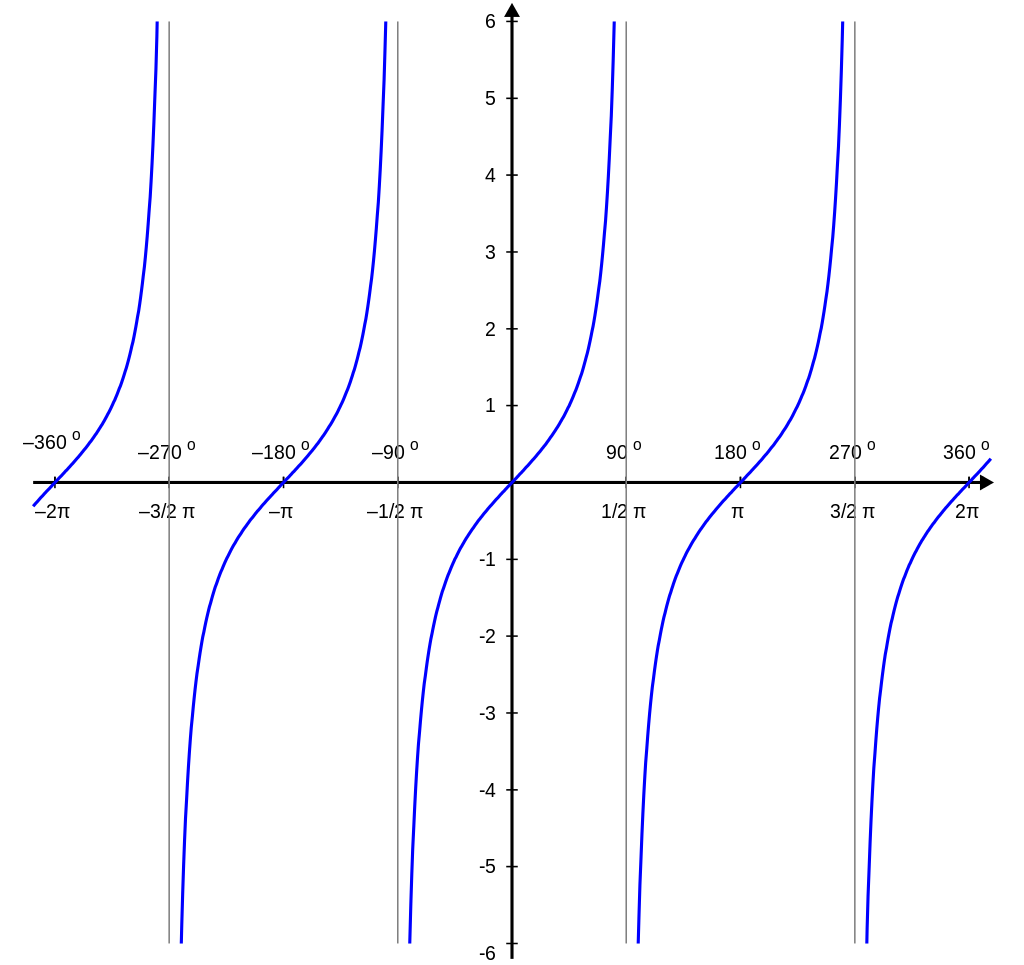
\includegraphics[width=0.9\linewidth]{Tan_proportional.png} 
        \caption{Tangensoida: wykres \\\hspace{\textwidth} funkcji $y = \tan x$}
        \label{fig:wykres-tangens}
    \end{minipage}%
    \begin{minipage}{0.5\textwidth}
        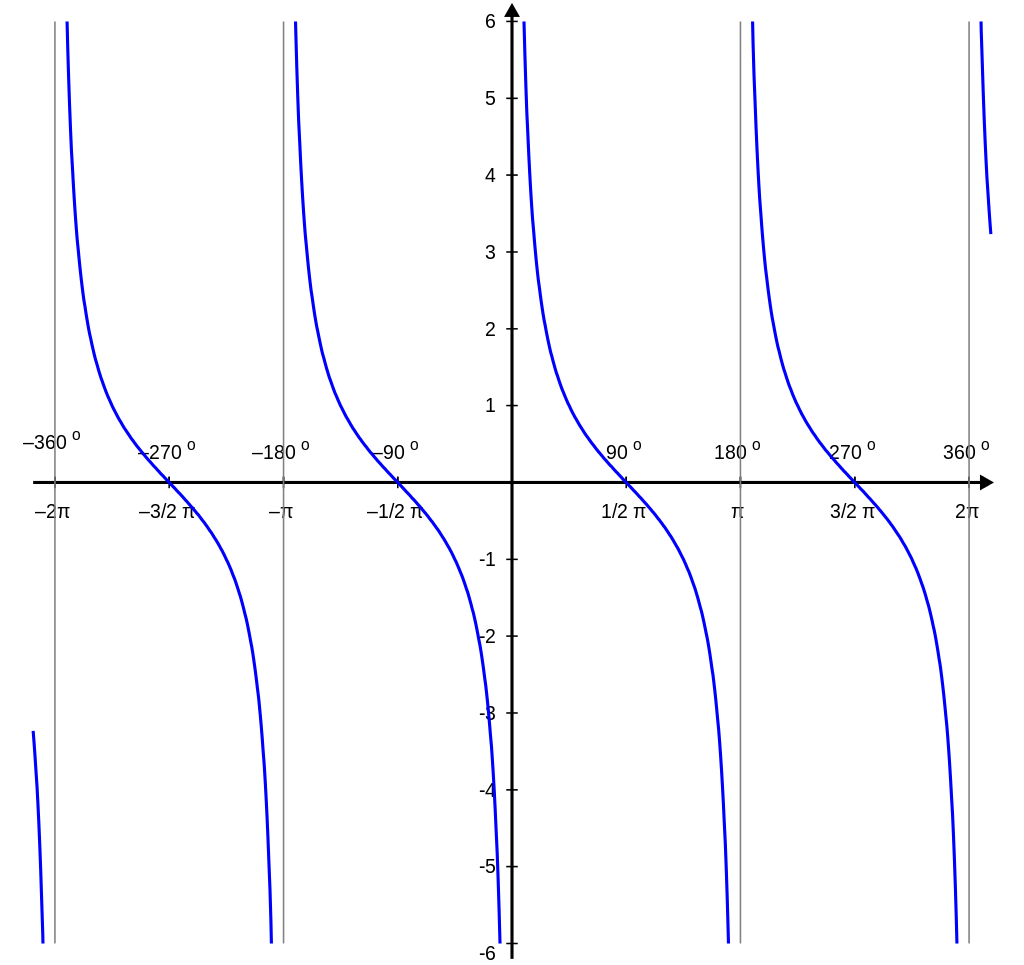
\includegraphics[width=0.9\linewidth]{Cotan_proportional.png}
        \caption{Cotangensoida: wykres \\\hspace{\textwidth} funkcji $y = \cot x$}
        \label{fig:wykres-cotangens}
    \end{minipage}
\end{figure}

\newpage

\section{Wartości dla typowych kątów}

\subsection{Wartości funkcji trygonometrycznych dla kątów $0, \frac{\pi}{6}, \frac{\pi}{4}, \frac{\pi}{3}, \frac{\pi}{2}, \pi$}

\bgroup
\setlength{\tabcolsep}{12pt}
\def\arraystretch{2.5}
\begin{table}[h]
\centering
    \begin{tabular}{|c|c|c|c|c|c|c|}
        \hline
        radiany & $0$ & $\dfrac{\pi}{6}$ & $\dfrac{\pi}{4}$ & $\dfrac{\pi}{3}$ & $\dfrac{\pi}{2}$ & $\pi$ \\ \hline
        $\sin$ & $0$ & $\dfrac{1}{2}$ & $\dfrac{\sqrt{2}}{2}$ & $\dfrac{\sqrt{3}}{2}$ & $1$ & $0$ \\ \hline
        $\cos$ & $1$ & $\dfrac{\sqrt{3}}{2}$ & $\dfrac{\sqrt{2}}{2}$ & $\dfrac{1}{2}$ & $0$ & $-1$ \\ \hline
        $\tan$ & $0$ & $\dfrac{\sqrt{3}}{3}$ & $1$ & $\sqrt{3}$ & $-$ & $0$ \\ \hline
        $\cot$ & $-$ & $\sqrt{3}$ & 1 & $\dfrac{\sqrt{3}}{3}$ & $0$ & $-$ \\ \hline
    \end{tabular}
    \caption{Tabela wartości funkcji trygonometrycznych}
    \label{tab:tabela-wartosci}
\end{table}
\egroup

\subsection{Znak wartości funkcji trygonometrycznych w poszczególnych ćwiartkach układu współrzędnych}

\bgroup
\setlength{\tabcolsep}{5pt}
\def\arraystretch{1.5}
\begin{table}[h]
\centering
    \begin{tabular}{|c|c|c|c|c|}
        \hline
         & I ćwiartka & II ćwiartka & III ćwiartka & IV ćwiartka \\ \hline
        $\sin$ & $+$ & $+$ & $-$ & $-$ \\ \hline
        $\cos$ & $+$ & $-$ & $-$ & $+$ \\ \hline
        $\tan$ & $+$ & $-$ & $+$ & $-$ \\ \hline
        $\cot$ & $+$ & $-$ & $+$ & $-$ \\ \hline
    \end{tabular}
    \caption{Tabela znaków funkcji trygonometrycznych w zależności od ćwiartki}
    \label{tab:tabela-znakow-funkcji}
\end{table}
\egroup

\newpage

\section{Własności funkcji trygonometrycznych}

\begin{enumerate}
    \item \textbf{Dziedzina}
    \begin{itemize}
        \item Funkcje sinus i cosinus określone są dla każdej liczby rzeczywistej.
        \item Tangens jest określony w zbiorze powstałym ze zbioru wszystkich liczb rzeczywistych przez usunięcie liczb mających postać $\frac{\pi}{2} + k\pi$, gdzie $k \in \mathbb{Z}$.
        \item Cotangens jest określony w zbiorze wszystkich liczb rzeczywistych poza liczbami postaci $k \pi$, gdzie $k \in \mathbb{Z}$.
    \end{itemize}
    
    \item \textbf{Przeciwdziedzina}
    \begin{itemize}
        \item Sinus i cosinus są ograniczone: przyjmują wartości z przedziału $[-1,1]$. Tangens i cotangens przyjmują dowolne wartości rzeczywiste.
    \end{itemize}
    
    \item \textbf{Ekstrema}
    \begin{itemize}
        \item Maksymalną wartość, dla obu funkcji $1$, sinus przyjmuje w punktach $x = \frac{\pi}{2} + 2k\pi$, a cosinus w punktach $x = 2k\pi$, gdzie $k \in \mathbb{Z}$.
        \item Maksymalną wartość, dla obu funkcji $-1$, sinus przyjmuje w punktach $x = -\frac{\pi}{2} + 2k\pi$, a cosinus w punktach $x = \pi + 2k\pi$, gdzie $k \in \mathbb{Z}$.
    \end{itemize}
    
    \item \textbf{Miejsca zerowe}
    \begin{itemize}
        \item Miejscami zerowymi sinusa i tangensa są punkty postaci $x = k\pi$, gdzie $k \in \mathbb{Z}$.
        \item Miejscami zerowymi cosinusa i cotangensa są punkty postaci $x = \frac{\pi}{2} + k\pi$, gdzie $k \in \mathbb{Z}$.
    \end{itemize}
    
    \item \textbf{Parzystość i nieparzystość}
    \begin{itemize}
        \item Funkcje sinus, tangens i cotangens są nieparzyste.
        \item Funkcja cosinus jest parzysta.
    \end{itemize}
    
    \item \textbf{Okresowość}
    \begin{itemize}
        \item Funkcje trygonometryczne są funkcjami okresowymi. 
        \begin{description}
            \item[$\sin, \cos$:] Okresem podstawowym sinusa i cosinusa jest liczba $2\pi$. Zobacz wykres \ref{fig:wykres-sinus} i \ref{fig:wykres-cosinus}.
            \item[$\tan, \cot$:] Okresem podstawowym tangensa i cotangensa jest liczba $\pi$. Zobacz wykres \ref{fig:wykres-tangens} i \ref{fig:wykres-cotangens}.
        \end{description}
    \end{itemize}
    
    \item \textbf{Ciągłość i różniczkowalność}
    \begin{itemize}
        \item Funkcje sinus i cosinus są ciągłe i różniczkowalne w każdym punkcie prostej rzeczywistej. Tangens i cotangens także są ciągłe i różniczkowalne w swoich dziedzinach.
    \end{itemize}

    \newpage
    
    \item \textbf{Odwracalność}
    \begin{itemize}
        \item Żadna z nich nie jest funkcją różnowartościową, a zatem nie istnieją funkcje odwrotne do funkcji trygonometrycznych w całej dziedzinie. W pewnych przedziałach funkcje te są jednak różnowartościowe i można tam określić funkcje do nich odwrotne.
    \end{itemize}
\end{enumerate}

\section{Spis rysunków i tabel}

\listoffigures
\listoftables

\end{document}